\documentclass[conference]{IEEEtran}

\usepackage{graphicx}

\usepackage{placeins}

\graphicspath{{Figures/}}



\begin{document}
	
	\title{I am a title (RO SLAM Methods/Implementation Survey) }
	
	
	
	\author{David Grabowsky}
	
	
	
	\markboth{IEEE Transactions On xxxl, Vol. XX, No. Y, Month 2018}{Grabowsky: RO SLAM}
	
	
	
	
	
	
	
	\maketitle
	
	
	
	
	
	\begin{abstract}
		
		
		
		
		
		This is my abstract, there are many like it, but this one is mine. Will fill this in once paper is written ****
		
		
		
		An survey of current the current implementations and methodologies used for solving the range only systematic and localization problem (RO-SLAM). 
		
		
		
	\end{abstract}
	
	
	
	
	
	
	
	\section{Introduction} 
	
	
	
	\section{range only sensors/tech}
	
	\section{Methods...}
	
	\subsection{EKF}
	
	%breif description (1-2 paragraphs)
	
	%paragraphs 
	
	The Extended Kalman Filter (EKF) is one of the most popular and widespread methods used to solve the SLAM problem. It is used to overcome the assumption of linear state transitions and measurements, which are rarely seen in practical environments \cite{Thrun2002}. The derivation of the EKF is very well documented, as such, detailed explanations can be viewed from a variety of sources such as: \cite{Thrun2002}, \cite{Ribeiro2004}, and \cite{Haykin2001}. When used to solve SLAM the map applied to the EKF is a feature based map, meaning it is composed of observable features (landmarks) which can be distinguished between during re-observation \cite{Thrun2002}. This distinction becomes important when examining range only SLAM (RO-SLAM) where only the range to a landmark, or the range between landmarks, is known. This restriction means that landmarks often need to be manufactured, such as those discussed in section II, and physically placed in an environment. However, that does not mean that the exact location of the landmarks, or even there initial existence, is recognized. Initialization is a critical element in many algorithms that make use of the EKF. If the initialization is inaccurate then the convergence to a correct estimation becomes much more difficult for the filter. The EKF has seen a wide variety of implementation ranging from ground based robotics\cite{Djugash2008}, to unmanned air vehicles \cite{Fabresse2016}, and to autonomous underwater vehicles \cite{Olson2006}. This section will proceed to give a summary of the various ways EKF has been implemented in regards to RO SLAM, as well as examine improvements to the general RO SLAM problem that are applied via EKF.
	
	
	
	A system for robust range only localization was prosed by \cite{Olson2006}. The system utilized an Autonomous Underwater Vehicle (AUV) and beacons without carefully surveyed locations. The paper notes that one of the majors issue was noise present in the received data. A method for outliers rejection caused by the noise was accomplished via spectral graph partitioning. A voting scheme was implemented similar to a Hugh transform to get approximate beacon locations \cite{Hough1959}. The approximate locations were then incorporated into an EKF. It is noted by the paper that this method is particularly CPU intensive, however they state that since the rate at which data is acquired from a landmark is slow, every 5 or so seconds, that the AUV can afford the expensive computation since there will be an adequate amount of time between readings for the data to process. The methodology was simulated using a dataset and can be seen in the paper.
	
	
	
	\cite{Kurth2003} presents a comparison of how three methods process a collected data set. The methods are a EKF, a sliding batch, and a particle filter. The comparison considers the cross-track error, and along track error. The results state that the particle filter works well when used to acquire an initial pose estimate, and EKF works well with real-time localization. It is suggested that in the future that the two could be switched between when appropriate to improve the overall system. 
	
	
	
	
	
	
	
	%fabreese. 
	
	%1. 2013 presents EKF slam method for ariel vehicles 
	
	%2. 2014 introduces prefiltering to measurments for previous 
	
	%3. 2014a integrates visual landmakrs as well
	
	%4  2015 decentralized multiple arieal vehicles
	
	%5  2016 specifically unmaned ariel, more details on 2013,2014 and experimental validation of 2013,2014.
	
	
	
	\cite{Vallicrosa2015} presents a solution utilizing a Sum of Gaussian (SOG) filter for a single range only beacon. It uses multivariate Gaussian mixtures to represent the probability distribution functions of the robot and beacon positions as Gaussian particles which each contain an EKF for vehicle position, velocity, and estimated beacon position. The paper presented experimentation where the method was used to map a beacon while correcting the navigation of the vehicle. 
	
	
	
	Several techniques have also been implemented that involve cooperative sensors. Traditionally sensors were used to only determine the range between themselves and the robot. The sensors in these cases provide the ability determine the range between themselves and other sensors and or the robot \cite{Patwari2005}.
	
	\begin{figure}[h!]
		
		\centering
		
		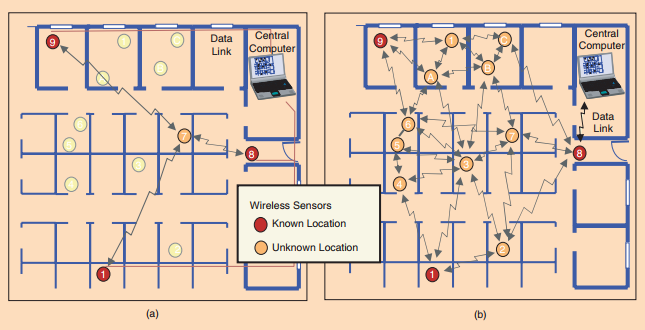
\includegraphics[width=90mm]{coop_loc_comp_patwari.png}
		
		\caption{Traditional(a) vs Cooperative(b) Sensors \cite{Patwari2005}}
		
		\label{trad_vs_coop_sensors}
		
	\end{figure}
	
	\FloatBarrier
	
	
	
	It is explained by \cite{Torres-Gonzalez2015} that methods utilizing inter beacon measurment should incorporate measurements with a configurable number of hops between beacons. This allows for the robot to gather range data from beyond the extent of the robots sensors. Experimentations was conducted utilizing this method via a particle filter EKF. The results showed that the more hops that were added the greater the performance of the system. 
	
	
	
	\cite{Djugash2006} presents a comparison of multiple RO SLAM methods utilized in two scenarios. One scenario involves the case where the robot only has access to range information between itself and beacons at unknown locations. In the second case the robot also has access to information about beacon to beacon distances. Several separate methods were compared in the given scenarios utilizing a data set and experimentation. The first method utilizes the Kalman filter in the case where only measurment between moving and stationary beacons are considered. Another method specifically uses the beacon to beacon measurements with an online Kalman filter. An off line batch method is used to get an estimate of the beacon location and robot path. Finally an method that considers the robot as a virtual node for creating submaps to be solved with a multidimensional scaling algorithm is also considered. The paper gives experimental results and analysis for each of the methods. 
	
	
	
	%In scenarios where the location of the landmarks is unknown and each landmark can not communicate with all every other landmarks, \cite{Djugash2006} presents a solution. He proposes that a moving beacon be used to add edges to the network \cite{Djugash2006}. In addition, no external position sensing were required on the part of the moving beacon, but the option for it to be incorporated was available. 
	
	
	
	
	
	
	
	
	
	
	
	
	
	One of the complications with RO-SLAM involves the issue of determining the location of landmarks when their initial placement is unknown, the EKF is sensitive to poorly initialized landmarks as they are used as the basis for the convergence of an accurate estimate. Caballero presents a solution for this complication. \cite{Caballero2010}. A Gaussian Mixture Model is integrated into the EKF to create a multiple hypothesis filter.  This multiple hypothesis approach is used to solve the RO-SLAM problem and its use allows for the un-delayed initialization of landmarks, however a large number of hypothesis can lead to increased computational burden. \cite{Geneve2015} also puts forward a method that utilizes a Gaussian mixtures for beacon initialization in EKF, but in this method only two hypotheses and a Cartesian plane are used.   \cite{Ahmad2011a} proposes to reduce the computational burden of methods such as the one proposed by Caballero \cite{Caballero2010} by introducing a novel state vector that eliminates the need for multiple hypothesis landmark representation. The paper proposes that under different circumstances the landmark could be represented using different parameters. Four circumstances are presented in the paper and the method is tested in simulation using both the EKF and a least squares optimization approach. The results showed that when the circumstances can be clearly distinguished between an increase in performance is seen.
	
	
	
	An extension to EKF called relative-over parametrized (ROP) EKF is presented by \cite{Djugash2008}. This extension uses specific parameterization to  better represent the range only data utilized in RO-SLAM. ROP EKF operates in polar coordinates as opposed to the Cartesian space that typical EKF operates. The method provided improved results over EKF when sparse range measurement of data association errors were present. \cite{Herranz2014} presents a comparison of the ROP-EKF method presented by \cite{Djugash2008}e{Djugash2008},to a smoothing and mapping method presented by \cite{Dellaert2006}. Experimentation conducted by Herranz on and indoor and outdoor environment show an improvement in the results of the SAM method over ROP EKF.
	
	\begin{figure}[h!]
		
		\centering
		
		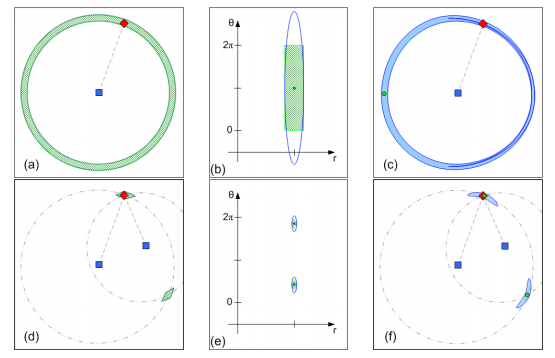
\includegraphics[width=90mm]{ROP_djugash.png}
		
		\caption{True and approximated distributions with one range observation (Top Row) and two observations from different locations (Bottom Row). True distributions in	Cartesian coordinates (Left Column), true and Gaussian approximated distributions in polar coordinates (Middle Column), and projection of the Gaussian approximated. \cite{Djugash2008}} LITERALLY COPIED, CHANGE DIS?%THIS WAS LITTERALY COPYIED AND PASTED AND NEEDS TO BE CHANGED AT SOME POINTS
		
		\label{ROP_djugash}
		
	\end{figure}
	
	\FloatBarrier
	
	
	
	
	
	A method proposed by \cite{Dios2015} is geared towards improving map building speed and accuracy for UAS dealing with the 3D RO-SLAM problem. The 3D RO-SLAM problem refers to the added complexity that devices such as submersibles \cite{Newman} and aerial vehicles experience when having to operate in an environment where three dimensions must be considered as opposed to the planar environment many robots are assumed to operate in. The method utilizes inter-beacon measurements and a novel mode selection which is used to select a measurement gathering method based on current conditions \cite{Dios2015}. The first mode is noted as mapping (MS) and the second localization (LS). When in mapping mode the measurment are integrated with a high probability to quickly create a map, when in localization mode the probability is lowered to create higher accuracy localizations. Based on experimentation performed by \cite{Dios2015} the method performed well an a general increase in accuracy and map speed was noted, however it is stated that a wider variety of experimentation should be performed to validate the overall robustness and effectiveness of the method.
	
	%this one might need some more work
	
	
	
	It is explored by \cite{Kehagias2006} how interpolation can be used to generate range data that is equally spaced over time as opposed to the irregular time intervals that range data is typically received at and then applied to solve the RO SLAM problem. The method is tested on the EKF and an batch optimization algorithm with a simulated and physical robot. The results provided show that the interpolation based algorithms gave better landmark estimation than those without, with the exception of the EKF in two datasets where EKF was already performing poorly.
	
	
	
	
	
	\cite{Fabresse2013} presents a solution for the 3D RO-SLAM problem. The solution reduces computational load through reduced spherical parametrization of map feature positions. The paper also proposes a new EKF update method which incorporates a reduced spherical representation of the state vector. In addition the paper describes how to efficiently integrate multi-modal belief of elevations angles and azimuth from a range sensor into the EKF utilizing two independent Gaussian Mixtures \cite{Fabresse2013}. In addition \cite{Fabresse2014} expands upon this by presenting a pre-filtering algorithm to be applied to range measurment before being used in the EKF in order to reduce the effect of noise generated by environmental issue such as multipathing. It is then proposed by \cite{Fabresse2015} that the above method can be utilized for decentralized multi-SLAM with range only sensors. This new method would allow for landmarks estimated by a robot to be incorporated into the estimation of another nearby robot, thus improving localization estimation. Based on experimental results obtained by \cite{Fabresse2015} the integration of estimates from multiple robots of the same landmarks provides a benefit to landmark localization over a single robot. In \cite{Fabresse2016} the author also validates and expands upon this method through indoor and outdoor experimentation with an Unmanned Aircraft System (UAS).  
	
	
	
	
	
	\subsection{Graph SLAM}
	
\subsection{Particle}      %change the references
Particles filters are made ue up various monte carlo algorithms that are used to estimate states in partially observable Markov chains(see[9]). In the initial application of particle filters in the field of robotics was in localization where it was used to estimate a robots pose from sensor data. It is considered better and more robust to conventional estimation methods because it was able to solve the global localization[2] and the kidnapped robot problem[14].It has also been at the corre higher dimensional problems  
%Description
Initially robot assumes global uncertainity through a set of particles that are distributed all over the map. Hence both the robot and the landmarks are uncertain.As the robot moves around and measures sensor data it resamples the particle set weighted according to the probability of the particle being the right one. There are several resampling methods depending on computational complexities. After some iterations only the particles which have a high degree of probability  reamain and eventually converge to the state of the robot and the landmarks.
\begin{figure}[h!]
	\centering
	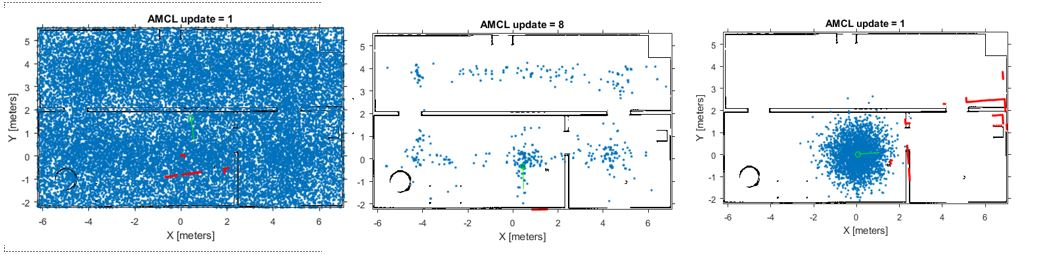
\includegraphics[height=40mm,width=90mm]{Particle_filter_method.JPG}
	\caption{The leftmost image describes the state of the robot when it just initializes the particle filter. The particles are uniformly distributed.The image in the center describes the particle filter after a couple of iterations. Only the particles which have a higher probability are re sampled. The image on the right shows the particle filter eventually converging to estimate the robot location. }
	
\end{figure}
Assuming at time t=0;we have N particles equally space in the enviornment that are drawn based on a uniform distribution $ p(x_oa)$.                                                                        resampling methods depending on computational complexities. After some iterations only th   p
Once the robot starts moving it collects measurements and at time $t>0$ we sample a new particle set $x^{[i]}_t$ for each particle in $x^{[i]}_{(t-1)}$. It is sampled based on the probability of measurement $p(z_t|x^{[i]}_{(t-1)})$. Eventually the particle filter converges to give us the true positioning of the robot.


As mentioned in[thrun particle] particle filters outperform EKF in applications involving global localization (the kidnapped robot problem form[14]) where the robot is randomly picked up and placed in a unknown environment. 
EKF cannot process negative information, but since particle filters use raw sensor data without any processing they can process negative information[thusn book[]
As the number of particles increases the computational complexity of the filter too increases. In order to address this there were several new methods introduced that  exploit the independence among state variables. For example the Rao-Blackwellized particle filters that exploit the independence of the landmarks with the robot path thereby reducing the computation complexity. from [Fast slam paper]. It also solves the data association problem previously unsolved by EKF.[8]
	
	
	
	\subsection{Graph}
	
	\subsection{Fast SLAM}
	
	%Brief introduction
	
	
	
	
	
	
	
	%advantages
	
	%Disadvantages
	
	
	
	
	
	\section{Conclusion}
	
	
	
	
	
	\bibliographystyle{IEEEtran}
	
	\bibliography{references}
	
	
	
\end{document}